\documentclass[20pt,,margin=1in,innermargin=-4.5in,blockverticalspace=-0.25in]{tikzposter}
\geometry{paperwidth=42in,paperheight=32.5in}
\usepackage[utf8]{inputenc}
\usepackage{amsmath}
\usepackage{amsfonts}
\usepackage{amsthm}
\usepackage{amssymb}
\usepackage{mathrsfs}
\usepackage{graphicx}
\usepackage{adjustbox}
\usepackage{SUtheme}
\usepackage{mathtools}
\usepackage{bm}
\usepackage{bbm}

\usepackage{mwe} % for placeholder images

% set theme parameters
\tikzposterlatexaffectionproofoff
\usetheme{SUTheme}
\usecolorstyle{SUStyle}
\usetitlestyle{Filled}

\usepackage[scaled]{helvet}
\renewcommand\familydefault{\sfdefault} 
\usepackage[T1]{fontenc}
% figure support
\usepackage{import}
\usepackage{xifthen}
\usepackage{pdfpages}
\usepackage{transparent}
\newcommand{\incfig}[1]{%
	\def\svgwidth{0.35\columnwidth}
	\import{./Figures/}{#1.pdf_tex}
}

\title{Using Graph Neural Network to Solve the Traveling Salesman Problem}
\author{Pingbang Hu, Jonathan Moore, Yi Zhou, Shubham Kumar Pandey, Anuraag Ramesh}
\institute{University of Michigan}
\titlegraphic{
\includegraphics[width=0.06\textwidth]{Figures/U-M_Logo-Hex.png}}

% begin document
\begin{document}
\maketitle
\centering
\begin{columns}
	\column{0.3}
	\block{Abstract}{
		\textbf{Graph neural network} is a rising concept in machine learning that has demonstrated significant potential in many areas.
		Our project aims to further explore this potential by applying it to the classic \textbf{Traveling Salesman Problem (TSP)}.
		We explore a novel concept called \textbf{imitation learning}, which is a special type of \textbf{reinforcement learning}.

		The former works focus on fixed-size training with large-size instances. In this work, we focus on the generalization ability of
		the model trained on small instances instead. Specifically, we train on TSP with 15
		nodes, which translate into an \textbf{Integer Linear Programming (ILP)} with hundreds of variables and
		several hundreds of constraints. Then, we test on TSP instances with instances of various sizes and see the generalization
		the ability of this novel approach.
	}

	\block{The Basics of GNN}{
		\textbf{A graph neural network (GNN)} is a class of neural networks for processing data best represented by graph structures.
		They were popularized by their use in supervised learning on properties of various molecules from the nature of this task: 3d graph
		structure.

		\par Since their inception, variants of the message passing neural network (MPNN) framework have been proposed. These models optimize
		GNNs for use on larger graphs and apply them to domains such as social networks, citation networks, and online communities. GNNs have
		also been relatively successful in various NP-hard combinatorial problems, automated planning and path-planning areas due to the
		inherent graph structure of data.
		\begin{center}
			\begin{minipage}{0.45\linewidth}
				\centering
				\begin{tikzfigure}
					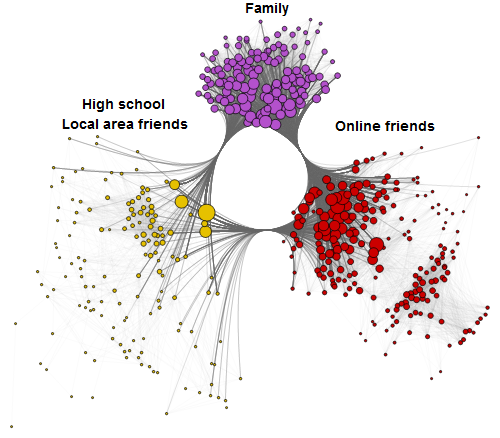
\includegraphics[width=13.6cm]{Figures/GNN_APP.png}
				\end{tikzfigure}%
			\end{minipage}\hfill
			\begin{minipage}{0.55\linewidth}
				\centering
				\begin{tikzfigure}
					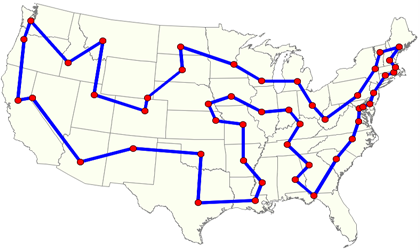
\includegraphics[width=14cm]{Figures/TSP.png}
				\end{tikzfigure}%
			\end{minipage}
		\end{center}
	}

	\block{Problem Formulation}{
		\textbf{One way} to formulate TSP is by \textbf{Integer Linear Programming}. Given an undirected weighted graph \(\mathcal{G} = (\mathcal{E}, \mathcal{V})\)
		with nodes being \(1, \ldots, n\), and define
		\[
			x_{ij}\coloneqq \begin{dcases}
				1, & \text{if }(i, j)\in \mathcal{E}^\ast                       \\
				0, & \text{if } (i, j)\in \mathcal{E}\setminus\mathcal{E}^\ast,
			\end{dcases}
		\]
		where \(\mathcal{E}^\ast\subset \mathcal{E}\) is a valid path in this TSP instance.
		This means that \(x_{ij}\) acts like an \textbf{indicator} variable. We further denote the weight on edge \((i, j)\) by \(c_{ij}\), then for a TSP problem
		instance, we can formulate the problem by so-called \textbf{Miller-Tucker-Zemlin formulation}.

		A popular way to solve an ILP is to first \textbf{relax} the integrality constraints by letting \(x_{ij}\in[0, 1]\). Then, we
		can divide the original relaxed LP into two sub-problems by \textbf{splitting the feasible region} according to \textbf{a chosen variable}
		that violates integrality constraints in the current relaxed LP solution \(\bm{x}^\ast\), say \(\bm{x}^\ast _i\), then
		\[
			\bm{x}_{i} \leq \left\lfloor \bm{x}_{i}^\ast \right\rfloor\lor \bm{x}_{i} \geq \left\lceil \bm{x}_{i}^\ast \right\rceil,\qquad \exists i\leq p\mid \bm{x}_{i} ^\ast \notin \mathbb{\MakeUppercase{z}}
		\]
		are two additional constraints in two sub-problems respectively. This gives us a recursive algorithm called \textbf{Branch and Bound}.
	}

	\column{0.4}
	\block{Learning Algorithm}{
	\textbf{A good branching} decision can reduce the sub-problem size, hence the solving time significantly since we
	can estimate the lower bound after each branching of the optimal cost. Then, after a branching, we can eliminate
	those branching choices are not going to produce a better tour.

	\textbf{Our goal now is to learn how to branch}. This is a sequential decision problem, hence, we naturally model
	this as a \textbf{Markov Decision Process (MDP)} problem. Surprisingly, this branching decision problem naturally
	has an \textbf{graph structure}, hence, rather than model TSP by a graph from nodes' coordinates, we
	\textbf{model the problem as a graph from a way deeper viewpoint}.

	\vspace{1em}
	\textbf{Our learning pipeline} is as follows. We first create some random TSP instances, and turn it into ILP.
	Then, we use imitation learning to learn how to choose the \textbf{branching target} at each branching.
	Our GNN model will produce a set of action with the probability corresponding to each possible action, in this
	case, which variable to branch. We then use \textbf{Cross Entropy Loss} to compare our prediction to the result
	produced by \texttt{SCIP} and complete one iteration.
	\begin{tikzfigure}
		\centering
		\incfig{pipeline}
	\end{tikzfigure}
	\textbf{Specifically}, we will pass TSP instances to \texttt{SCIP}, which is a modern SOTA MILP (Mixed Integer Linear Programming) solver, to get all
	the solving states in order to solve MDP problem. The modern solver usually uses mixed branching strategy to balance the running
	time, and a well-known costly but strong strategy is called \textbf{strong branching}, and in order to learn the strongest branching strategy, we make
	\texttt{SCIP} to use strong branch with probability a half. This learning process is called \textbf{imitation learning}, or \textbf{behavioral
		cloning}.

	Mathematically, we first run the SOTA solver \texttt{SCIP} to get state-action pairs \(\mathcal{\MakeUppercase{d}} = \left\{(s_{i} , \bm{a} _{i} ^\ast)\right\}_{i = 1}^N\),
	where the state is the solver's branching strategy, and the action set contains what variables we can branch on.


	To learn the policy \(\widetilde{\pi} ^\ast\), we minimize the cross-entropy loss between our branching prediction and the solver's branching choice:
	\[
		\mathcal{\MakeUppercase{l}} (\theta ) = - \frac{1}{N}\sum\limits_{(\bm{s}, \bm{a}^\ast)\in \mathcal{\MakeUppercase{d}} }\log \widetilde{\pi}_\theta (\bm{a} ^\ast \mid \bm{s} ).
	\]

	After learning, we evaluate our model on TSP instances with various sizes to see the generalization ability. Specifically, we use
	Ecole to do the evaluation. We configure \texttt{SCIP} to its default strategy and compare the result to our learned branching
	strategy by looking at the time needed to solve this particular TSP instance.
	}

	\column{0.3}
	\block{Experimental Result}{
		We test the generalization ability of our model trained with TSP15 on various sizes TSP
		instances on GreatLakes with one A100 GPU and 8GB, 16 cores CPU. The figures below plots the
		walltime needed for our model and \texttt{SCIP} to solve a particular TSP instance on y-axis,
		and we do this for 100 instances for every testing size.
		\begin{center}
			\begin{minipage}{0.49\linewidth}
				\centering
				\begin{tikzfigure}
					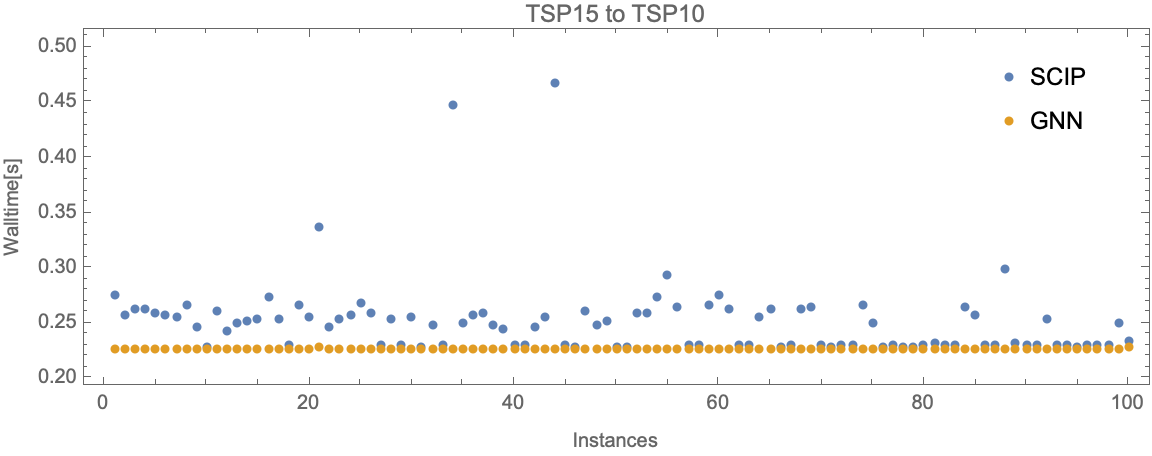
\includegraphics[width=13cm]{Figures/result/15-10(from15-20).png}
				\end{tikzfigure}%
			\end{minipage}\hfill
			\begin{minipage}{0.49\linewidth}
				\centering
				\begin{tikzfigure}
					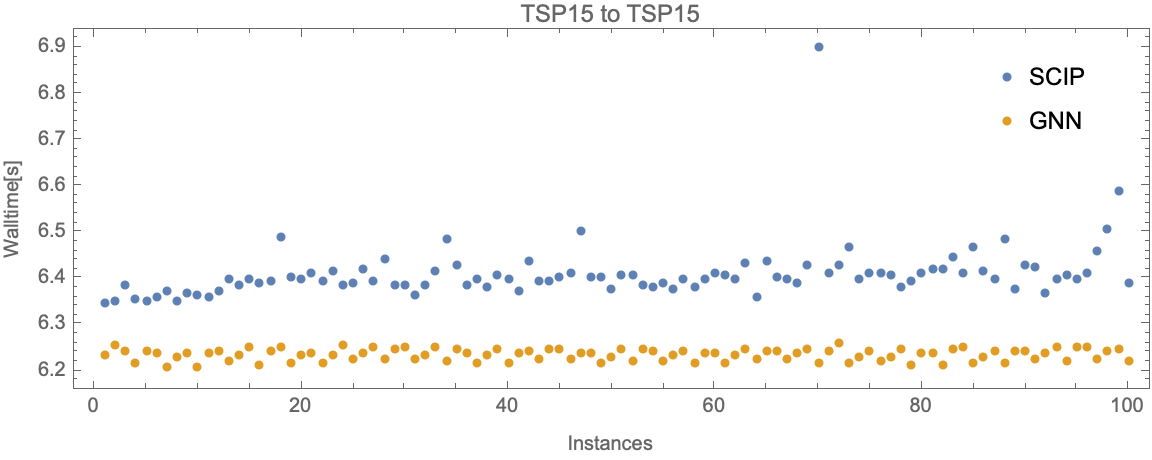
\includegraphics[width=13cm]{Figures/result/15-15.png}
				\end{tikzfigure}%
			\end{minipage}
			\begin{minipage}{0.49\linewidth}
				\centering
				\begin{tikzfigure}
					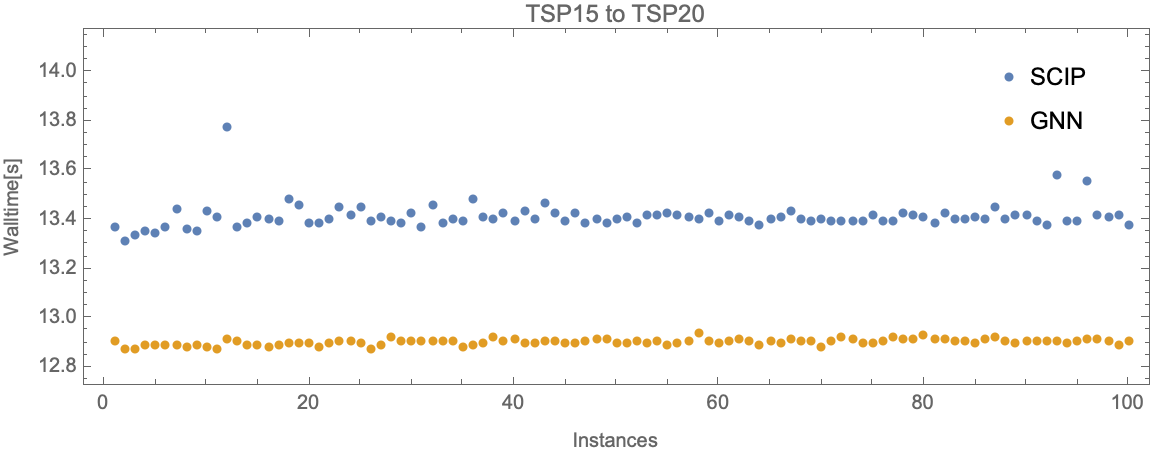
\includegraphics[width=13cm]{Figures/result/15-20.png}
				\end{tikzfigure}%
			\end{minipage}\hfill
			\begin{minipage}{0.49\linewidth}
				\centering
				\begin{tikzfigure}
					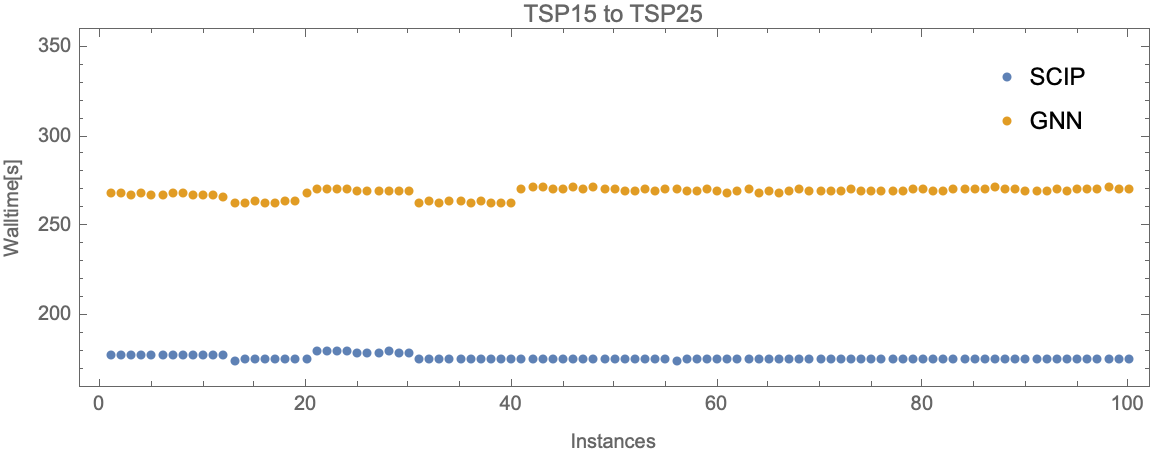
\includegraphics[width=13cm]{Figures/result/15-25.png}
				\end{tikzfigure}%
			\end{minipage}
			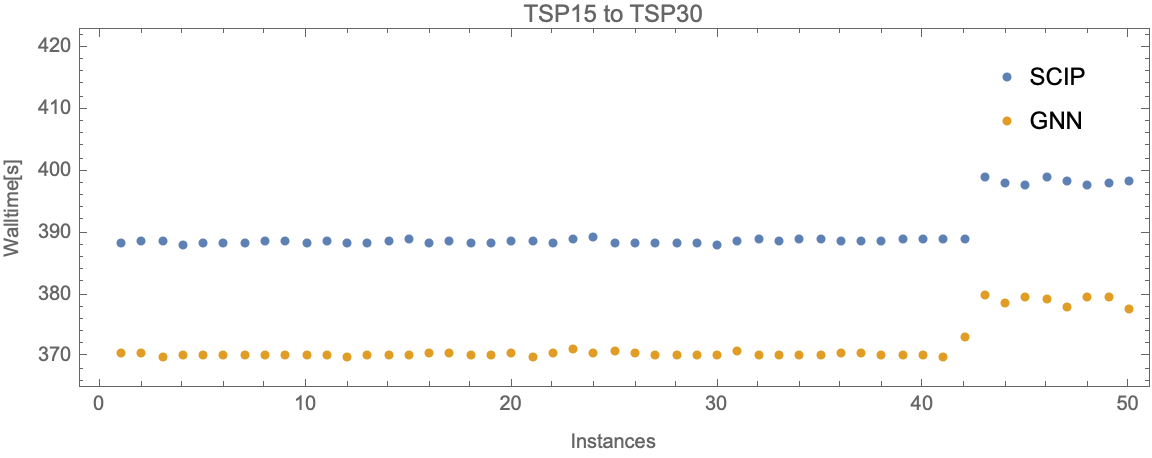
\includegraphics[width=27cm]{Figures/result/15-30(from15-15).png}
		\end{center}
		We see that our model outperform the baseline on TSP15, and \textbf{successfully generalize to TSP10, TSP20
			and TSP30}.

		However, there is a counter-intuitive result, namely on TSP20 and TSP30. We see that our model does not
		outperform the baseline, and is behind by 50\%\ on average; but our model does outperform the baseline
		by 4.70\%. A potential explanation is that our learned model is more stable and robust than the
		baseline's heuristic, hence we can still conclude that our model \textbf{do} generalize greatly on larger
		or smaller instances.
	}

	\block{Conclusion}{
		\textbf{Unlike other works} which focuses on just to solve TSP approximately, we focus on generalization ability of solving TSP \textbf{exactly}.

		With limited computation power and training on small size instances, our result shows a promising performance on the generalization ability of branch, which is a hard
		combinatorial optimization problem and typically hard to generalize.

		\textbf{The significance} of our works is pretty straightforward: We're now the confidence to generalize on larger instances by combining various machine learning techniques
		like standard reinforcement learning, deep learning, transformer, etc.
	}

	\block{Future Work}{
		\textbf{Due to computational limitation}, we can't train on larger instances. One may further generalize our work by training on larger instances, for instance, TSP50, TSP100, or higher.

		On the other hand, our work should be easy to reproduce and be combined with various standard reinforcement techniques to further fine-tuned our trained model.
	}
\end{columns}
\end{document}